\documentclass[a4j,twocolumn,10pt]{jarticle}
\usepackage{dia2022}
\usepackage{color}

\makeatletter
%%%タイトル調整
\setcounter{totalnumber}{3}
\def\id#1{\def\@id{#1}}
\def\@maketitle{%
\vspace{-4.3em}
\begin{center}%
{\@title \par}% タイトル
{\@author}% 著者
\end{center}%
%\par\vskip 1.5em
}
\makeatother

\title{
\vspace{15mm}
\Large{
\textbf{\leftline{【若手研究奨励賞候補:はい】}}\\
\textbf{機械学習による実環境下の変形ARマーカの位置・姿勢推定}} %%%%%%論文タイトルを記入
}

\author{
\vspace{1.5em}
\large{○榎元洋平 $\dagger$,} %%%%著者1->著者名1に書き換え,【重要】講演者に○を付けてください!
\large{山内悠嗣 $\ddagger$}\\                 %%%%著者2->著者名2に書き換え
\vspace{1em}
\large{{\rm ○ Yohei ENOMOTO $\dagger$\ }             %%%%Author1->著者名1ローマ字に書き換え
{\rm and\ }
{\rm Yuji YAMAUCHI $\ddagger$} }\\     %%%%Author2->著者名2ローマ字に書き換え
\vspace{0.5em}
\large{$\dagger$:中部大学,}     %%%%所属1->著者1の所属に書き換え
{\rm tr21004-4551@sti.chubu.ac.jp} \\                    %%%%著者1のメールアドレス
\large{$\ddagger$:中部大学,}    %%%%所属2->著者2の所属に書き換え
{\rm yuu@isc.chubu.ac.jp }\\                     %%%%著者2のメールアドレス
}
\date{} %日付を表示しない
\pagestyle{empty}

\setstretch{1.1} %%%行間隔調整用:適宜調整してください.
%\pagestyle{empty}
\begin{document}
%---タイトル---
\twocolumn[
\maketitle
\thispagestyle{empty} %maketitleをいじっている関係でここでページ番号を消去
\vspace{-2em}
\begin{abstract}
 \noindent{}<要約>本論文では変形したARマーカの検出と位置・姿勢推定方法を提案する.実空間上のARマーカを評価するため機械学習を用いて変形したARマーカの検出と姿勢推定し,カメラで撮影されたARマーカの大きさより位置推定する.\\
 <キーワード>6DoF,物体認識,オートエンコーダ,機械学習
\vspace{2.5em}
\end{abstract}]
\vspace{1em}

%--- 本文開始 ---
\section{はじめに}
近年,ARマーカが普及しゲームやカタログ,ドローンの制御にも活用されている.
ARマーカを認識し,位置・姿勢を推定することで様々なコンテンツを利用できる.
そのため,ARマーカの位置・姿勢の推定精度が求められている.
しかし,ARマーカに変形が生じるとARマーカの認識精度は低下し,位置・姿勢の推定も困難になる.
そこで,本研究では,機械学習によって変形したARマーカを実環境下で認識し位置・姿勢の推定方法を提案する.

\section{提案手法}
本研究は,変形したARマーカの検出,姿勢の推定,位置の推定により構成される.
なお,本稿では円柱に貼り付けることにより変形したARマーカを変形ARマーカとして扱う.


\subsection{変形ARマーカの検出}
Single Shot Multibox Detector(SSD)[1]によって変形ARマーカを検出する.SSDは画像から物体の位置とクラスを推定する物体検出アルゴリズムである.
SSDの学習用画像とアノテーションデータをロボットシミュレータGazeboにより作成する.
仮想空間内で変形ARマーカを表示させ,仮想カメラで様々な視点から撮影し学習用画像とアノテーションデータを生成した.
学習用画像とアノテーションデータを用いて,変形ARマーカの検出とマーカIDを出力する検出器を学習する.



\subsection{変形ARマーカの姿勢推定}
Augmented AutoEncoder(AAE)[2]によって変形ARマーカの姿勢推定をする.
まず,Gazeboにより変形のないARマーカ画像(図1.(a))と変形AR マーカ画像(図1.(b))を生成する. 
そして,変形ARマーカ画像をオートエンコーダに入力し,変形を除去したARマーカ画像 (図1.(c))を生成する.
変形のないARマーカ画像と変形を除去したARマーカ画像の違いを吸収するようなオートエンコーダを学習させる.
%式(1)で示す損失関数$L$を最小化する. 
%\vspace{-1.0zh}
%\begin{eqnarray}
%\label{sonsitu}
%L=\frac{1}{n} \sum_{i=1}\left\|x_{i}-x_{i}^{\prime}\right\|_{2}
%\end{eqnarray}
%\vspace{-2.1zh}

%$x$は変形を含まない画像,$x'$はオートエンコーダにより出力した画像を表す.

\vspace{-1.3zh}
\renewcommand{\arraystretch}{1.0}
\begin{figure}[h]
\centering
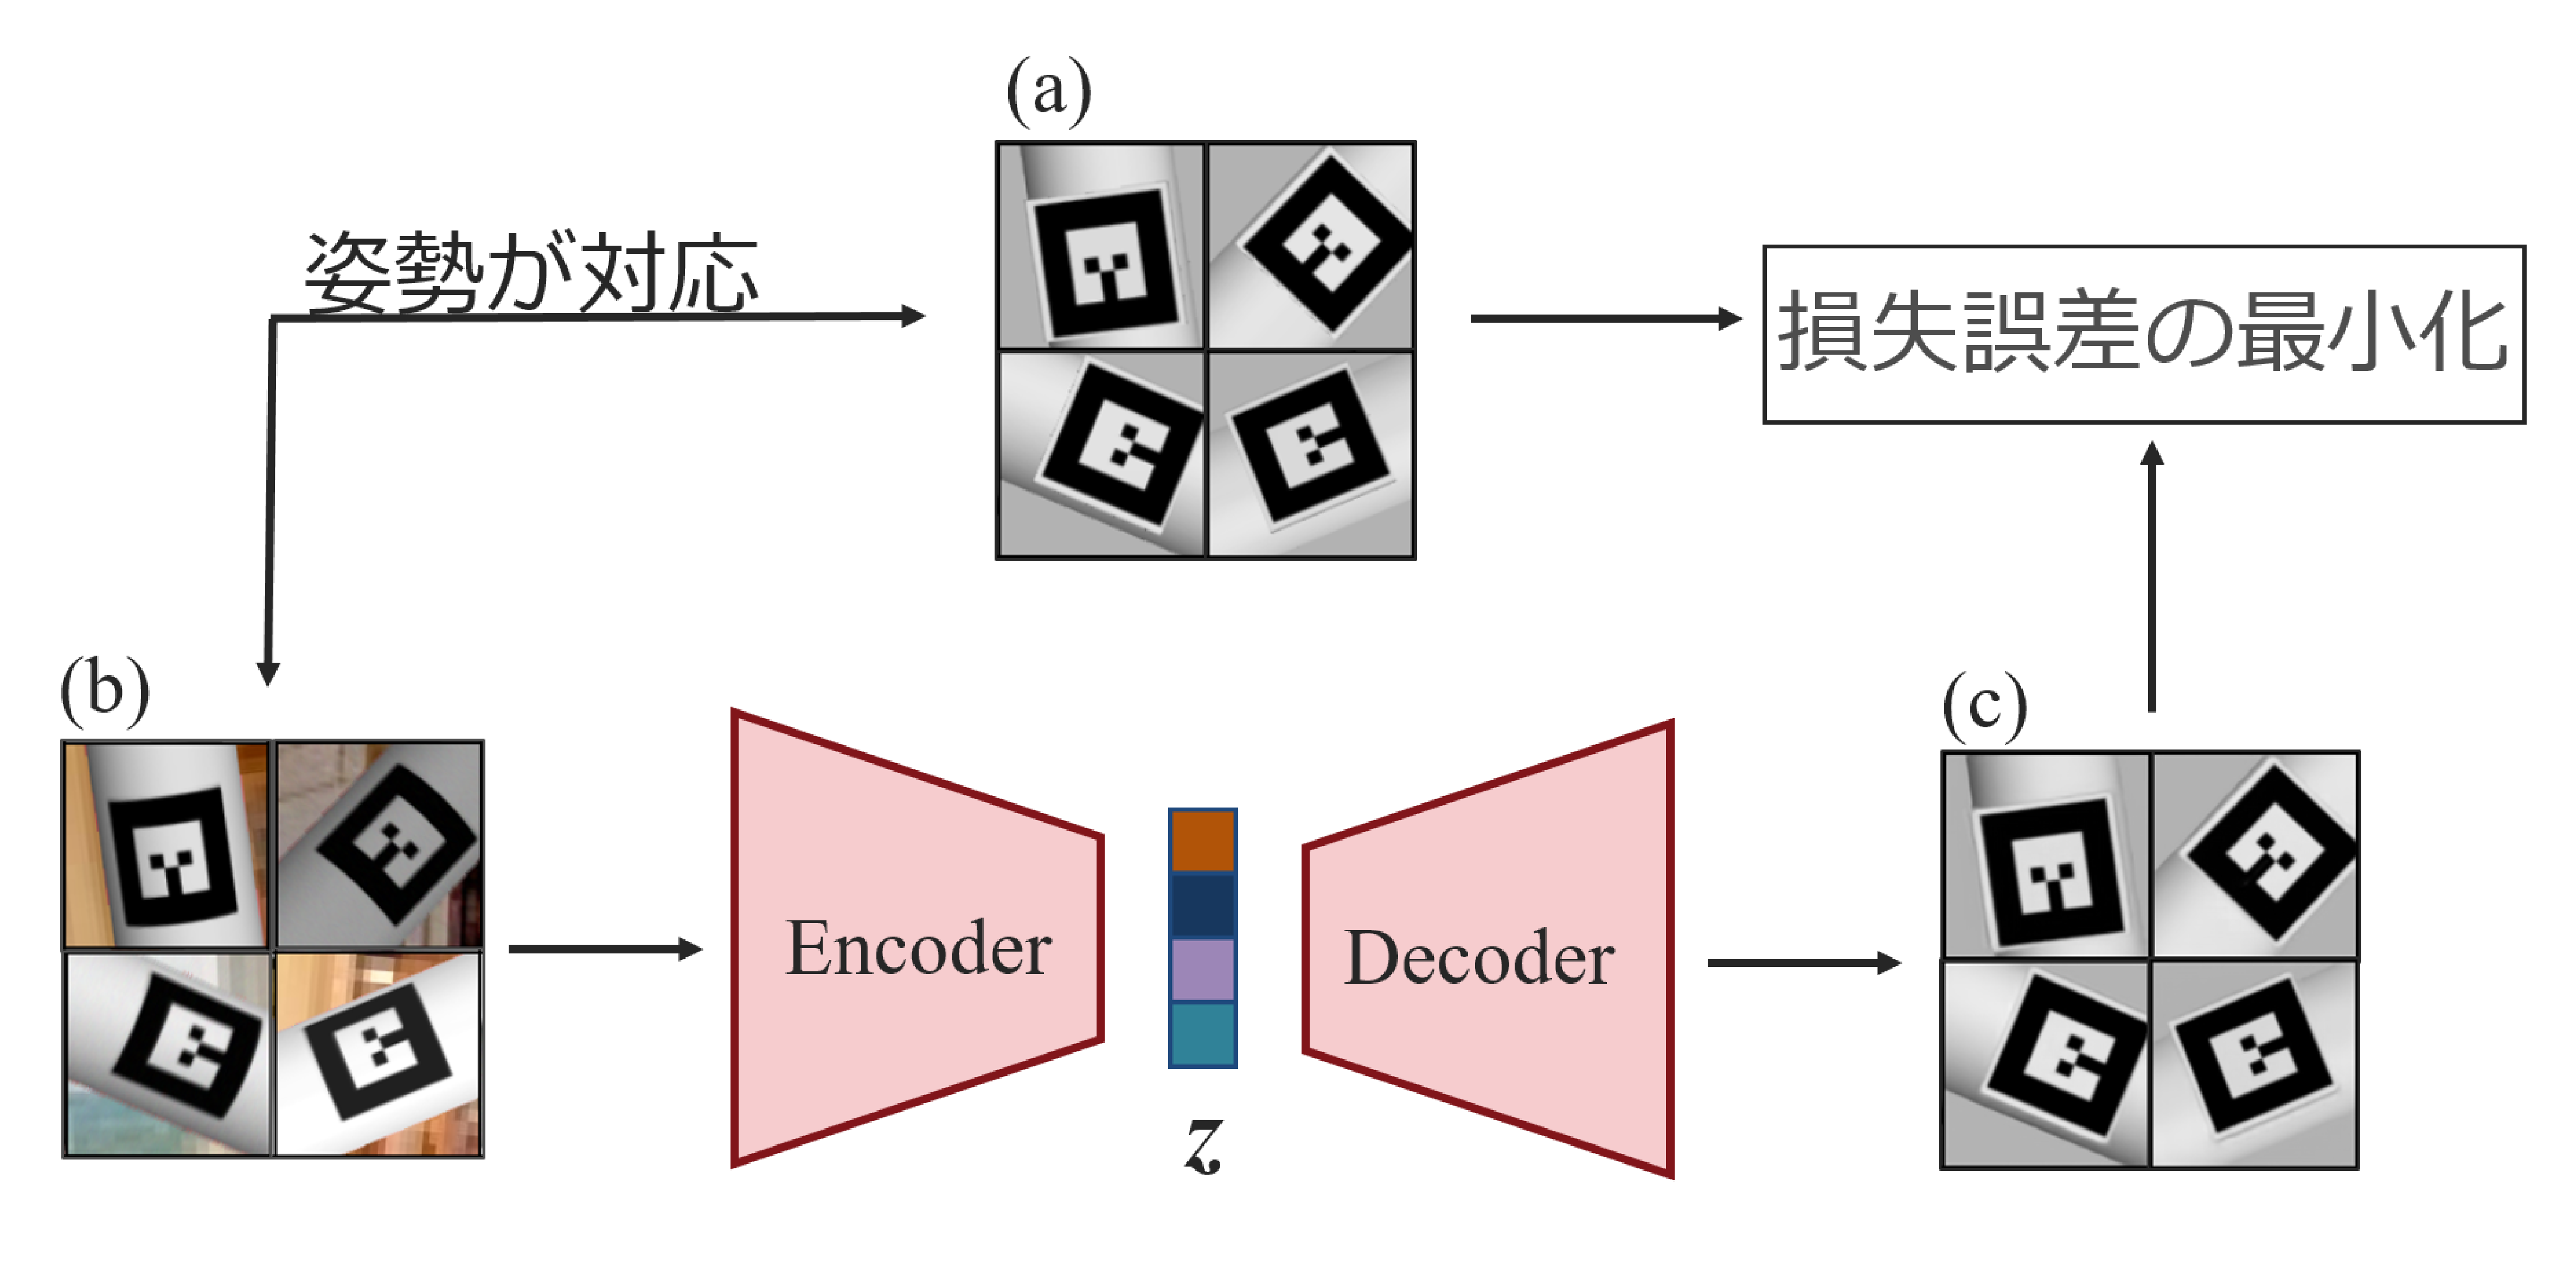
\includegraphics[width=65mm]{./画像/AAE.eps}
\caption{AAEの概要}
\label{fig:graph3}
\end{figure}
\vspace{-1.0zh}

変形が生じたARマーカの姿勢は,入力画像をエンコーダに入力して得られる潜在変数$z$に基づいて推定する.
事前にARマーカの姿勢をroll[0,360],pitch[-14,14],yaw[-14,14]を分解能1[$°$]に設定して変形ARマーカをGazeboで撮影し,姿勢データベース(DB)の潜在変数群$Z$として用意する.テスト時には,SSDにより検出した変形ARマーカをAAEに入力することで得られる潜在変数とDBの潜在変数群のコサイン類似度を求め,最も類似度が高い潜在変数を求める.
そして,求めた潜在変数に対応した姿勢を出力する. 


\subsection{変形ARマーカの位置推定}

カメラから物体までの並行ベクトルを求める手法[3]により変形ARマーカの三次元位置を推定する.
まず,変形ARマーカをSSDに入力し,変形ARマーカが検出され,Bounding box(Bbox)で囲まれる.入力した変形ARマーカのBboxの大きさと仮想空間内で撮影された変形ARマーカのBboxの大きさより奥行きベクトル$\hat{t}_{real,z} $を式(1)より算出する.
\vspace{-1.2zh}
\begin{eqnarray}
\label{sonsitu}
\hat{t}_{real,z}=t_{syn,z} \times \frac{\left\|b b_{ {syn},argmax(\cos_{i})}\right\|} {\left\|b b_{{real}}\right\|} \times \frac{f_{{real}}}{f_{{syn }}}
\end{eqnarray}
\vspace{-2.7zh}


仮想空間内で撮影されたDBの変形ARマーカの奥行き方向の距離$t_{syn,z}$,
SSDから検出された変形ARマーカのBboxの対角線の最大値$b b_{{syn},{argmax}\left(\cos _{i}\right)}$,仮想空間内で撮影されたDBの変形ARマーカのBboxの対角線の大きさ${b b_{real}}$,
実環境と仮想空間内の撮影に使用したカメラの焦点距離$f_{{real}}$,$f_{{syn}}$とする.\par 
次に式(2)によって平行ベクトル$\Delta \boldsymbol{\hat{t}}$を求める.

\vspace{-3.0zh}
\begin{eqnarray}
\label{sonsitu}
\Delta \boldsymbol{\hat{t}}=\hat{t}_{real,z} \boldsymbol{{K}_{real}^{-\mathbf{1}}} \boldsymbol{b} \boldsymbol{{b}_{real,c}}-t_{syn,z} \boldsymbol{{K}_{syn}^{-\mathbf{1}}} \boldsymbol{{b}} \boldsymbol{{b}_{syn,c}}
\end{eqnarray}
\vspace{-2.7zh}

実環境と仮想空間内の撮影に用いたカメラのカメラ行列$\boldsymbol{{K}_{real}^{-\mathbf{1}}}$,$\boldsymbol{{K}_{syn}^{-\mathbf{1}}}$,実環境と仮想空間内の変形ARマーカの検出した際に得られるBboxの中心座標$\boldsymbol{b} \boldsymbol{{b}_{real,c}}$,$\boldsymbol{{b}} \boldsymbol{{b}_{syn,c}}$とする.
最後にDB内の変形ARマーカの中心座標と求めた$\Delta \boldsymbol{\hat{t}}$によって位置を推定する.

%\vspace{-2.2zh}
%\begin{eqnarray}
%\label{sonsitu}
%\boldsymbol{\hat{t}_{real }} = \boldsymbol{{t}_{syn}}+\boldsymbol{\Delta \hat{t}}
%\end{eqnarray}
%\vspace{-3.2zh}

\section{評価実験}
提案手法の有効性を確認するために評価実験を行う.
一辺50[mm]のARマーカ10種類を半径20,30,40[mm]の円柱に貼り付け変形させたARマーカを実環境で撮影する.
撮影した画像を提案手法に適用し検出精度,姿勢推定,位置推定の評価する.

\subsection{変形ARマーカの検出結果}
SSDによる変形ARマーカの検出精度を検証する.
評価指標として,マーカの認識精度にはmean Average Precision(mAP)とARマーカの位置の検出精度にはIntersection over Union(IoU)を採用する.
検出結果はmAPが0.98,IoUが0.89となり実環境下でも高精度な検出が可能である.

\subsection{変形ARマーカの位置・姿勢推定精度}
変形ARマーカの位置・姿勢推定の結果を平均絶対誤差(MAE)により評価する.
姿勢推定は変形ARマーカをSSDにより検出し,ARマーカを中心として一定領域を切り出した画像を評価する.
位置推定は変形ARマーカをSSDにより検出した際に得られるBboxの大きさから評価する.
\par 
姿勢推定の評価結果を表1に示す.
提案手法による三次元姿勢推定のMAEは3.47[$°$]である.誤差はあるが姿勢推定可能である.


\begin{table}[h]
        \vspace{0zh}
          \begin{center}
            \caption{提案手法における姿勢推定誤差}
            \vspace{-1zh}
            \label{hyouka}
            \begin{tabular}{c|c|c|c|c} \hline
              円柱半径[mm]   & roll& pitch & yaw&平均 \\ \hline
              20& 5.4 & 4.3 & 5.1 &4.93\\ \hline
              30&4.7 & 3.2 & 3.4& 3.76 \\ \hline
              40&2.4 &1.4  &1.4&1.73 \\ \hline
              \end{tabular}
          \end{center}
        \vspace{-2zh}
\end{table}

円柱の半径が小さいほどMAEが大きくなる傾向が得られた.これは円柱の半径が小さいほどARマーカの変形が大きいためだと考えられる.\par 
次に位置推定の評価結果を表2に示す.
提案手法による三次元位置推定のMAEは0.038[m]である.結果より位置推定が可能である.

\begin{table}[h]
        \vspace{0zh}
          \begin{center}
            \caption{提案手法における位置推定誤差}
				\vspace{-1zh}
            \label{hyouka}
            \begin{tabular}{c|c|c|c|c} \hline
              円柱半径[mm]   & x& y & z&平均 \\ \hline
              20& 0.06 & 0.03 & 0.03 & 0.04\\ \hline
              30& 0.05 & 0.02 & 0.04 & 0.036 \\ \hline
              40& 0.05 & 0.02 & 0.03 & 0.033 \\ \hline
              \end{tabular}
          \end{center}
        \vspace{-2zh}
\end{table}

図2に提案手法によって位置・姿勢を推定した例を示す.変形したARマーカでも高精度に位置・姿勢の推定が可能であることが分かる.

\renewcommand{\arraystretch}{1.0}
\begin{figure}[h]
\vspace{-1zh}
\centering
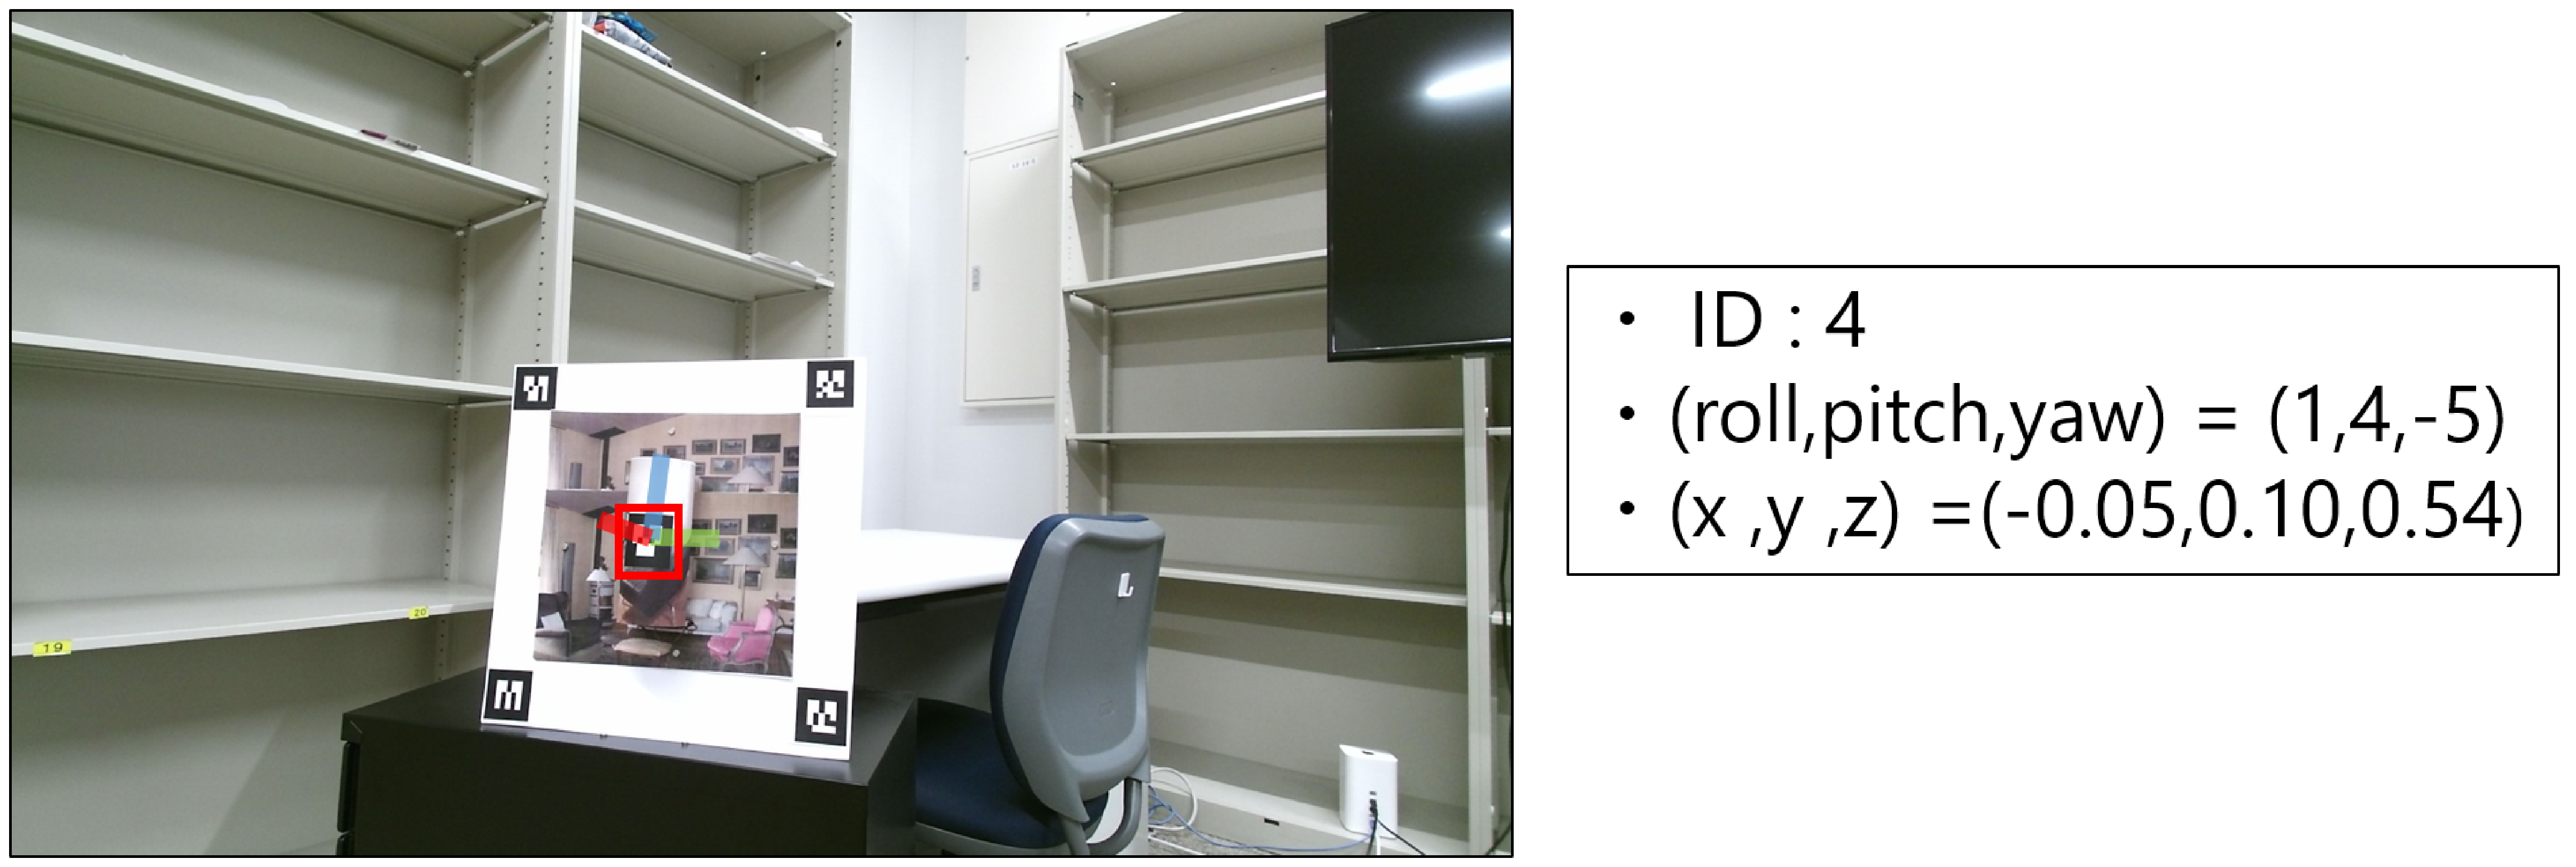
\includegraphics[width=87mm]{./画像/推定結果.eps}
\caption{推定結果の例}
\label{fig:graph3}
\vspace{-2zh}
\end{figure}



\section{おわりに}
本研究では,実環境下における変形ARマーカの検出及び位置・姿勢推定方法を提案した.今後は画像1枚に対する処理速度を向上させる予定である.


\markboth{参考文献}{}     %% BibTeX を使う

\begin{thebibliography}{1}

{\scriptsize \bibitem {1} W.Liu et al.                     :“SSD: Single Shot MultiBox Detector”,ECCV,2016.}
{\scriptsize \bibitem {2} Kehl W et al.                   :“SSD-6D: Making RGB-Based 3D Detection and 6D Pose Estimation Great Again”,ICCV,2017.}
{\scriptsize \bibitem {3} Martin Sundermeyer et al. :“Implicit 3D Orientation Learning for 6D Object Detection from RGB Images”,ECCV,2019.}

\end{thebibliography}
\end{document}

\end{document}
